\documentclass[11pt,a4paper]{article}
\usepackage[T1]{fontenc}
\usepackage[utf8]{inputenc}
\usepackage{lmodern}
\usepackage[margin=2.5cm]{geometry}
\usepackage{amsmath}
\usepackage{booktabs}
\usepackage{graphicx}
\usepackage{caption}
\usepackage[hidelinks]{hyperref}
\usepackage{xcolor}
\usepackage[round]{natbib}
\captionsetup{font=small,labelfont=bf}
\graphicspath{{../figures/}}
% Generated by src/10_paper_numbers.py. Do not edit.
\newcommand{\NEpisodes}{9}
\newcommand{\NPulls}{3}
\newcommand{\NDraws}{2,000}
\newcommand{\NPoolWeeks}{66}
\newcommand{\AnchorValidityP}{0.566}
\newcommand{\ThrUK}{25.5}
\newcommand{\ThrEngland}{26.2}
\newcommand{\ThrScotland}{21.6}
\newcommand{\ThrWales}{24.5}
\newcommand{\ThrNI}{22.8}
\newcommand{\MaxDose}{34.7}
\newcommand{\MaxDoseEpisode}{22 June 2026}
\newcommand{\DoseJulyTwentyTwo}{19.5}
\newcommand{\CalRMin}{0.986}
\newcommand{\CalRMax}{0.996}
\newcommand{\SparseHeatwave}{0.61}
\newcommand{\SparseCopingMin}{0.25}
\newcommand{\SparseCopingMax}{0.93}
\newcommand{\PullCorrMin}{0.92}
\newcommand{\WikiUKPass}{1}
\newcommand{\SizeAOneMin}{15}
\newcommand{\SizeAOneMax}{16}
\newcommand{\SizeATwo}{19}
\newcommand{\ImpSal}{0.62}
\newcommand{\ImpSalPct}{86}
\newcommand{\ImpSalRI}{0.012}
\newcommand{\ImpSalMDE}{0.64}
\newcommand{\ResSal}{$-$0.19}
\newcommand{\ResSalRI}{0.329}
\newcommand{\DecSal}{$-$0.09}
\newcommand{\LeadsSal}{0.741}
\newcommand{\ImpCop}{0.68}
\newcommand{\ImpCopPct}{97}
\newcommand{\ImpCopRI}{0.011}
\newcommand{\ImpCopMDE}{0.68}
\newcommand{\ResCop}{$-$0.07}
\newcommand{\ResCopRI}{0.714}
\newcommand{\DecCop}{$-$0.19}
\newcommand{\LeadsCop}{0.006}
\newcommand{\ImpCon}{0.30}
\newcommand{\ImpConPct}{35}
\newcommand{\ImpConRI}{0.018}
\newcommand{\ImpConMDE}{0.35}
\newcommand{\ResCon}{$-$0.07}
\newcommand{\ResConRI}{0.193}
\newcommand{\DecCon}{$-$0.04}
\newcommand{\LeadsCon}{0.672}
\newcommand{\ImpConPlan}{0.26}
\newcommand{\ImpConPlanPct}{30}
\newcommand{\ImpConPlanRI}{0.057}
\newcommand{\ImpConPlanMDE}{0.39}
\newcommand{\ResConPlan}{$-$0.10}
\newcommand{\ResConPlanRI}{0.069}
\newcommand{\DecConPlan}{$-$0.05}
\newcommand{\LeadsConPlan}{0.778}
\newcommand{\ImpWikiSal}{0.34}
\newcommand{\ImpWikiSalPct}{40}
\newcommand{\ImpWikiSalRI}{$<$0.001}
\newcommand{\ImpWikiSalMDE}{0.27}
\newcommand{\ResWikiSal}{0.04}
\newcommand{\ResWikiSalRI}{0.721}
\newcommand{\DecWikiSal}{0.11}
\newcommand{\LeadsWikiSal}{0.461}
\newcommand{\ImpWikiCon}{0.24}
\newcommand{\ImpWikiConPct}{27}
\newcommand{\ImpWikiConRI}{0.035}
\newcommand{\ImpWikiConMDE}{0.32}
\newcommand{\ResWikiCon}{$-$0.01}
\newcommand{\ResWikiConRI}{0.927}
\newcommand{\DecWikiCon}{$-$0.04}
\newcommand{\LeadsWikiCon}{$<$0.001}
\newcommand{\ImpWikiCop}{0.11}
\newcommand{\ImpWikiCopPct}{12}
\newcommand{\ImpWikiCopRI}{0.042}
\newcommand{\ImpWikiCopMDE}{0.16}
\newcommand{\ResWikiCop}{$-$0.02}
\newcommand{\ResWikiCopRI}{0.719}
\newcommand{\DecWikiCop}{$-$0.02}
\newcommand{\LeadsWikiCop}{0.243}
\newcommand{\ImpCarIns}{0.02}
\newcommand{\ImpCarInsRI}{0.528}
\newcommand{\ImpRecipes}{$-$0.04}
\newcommand{\ImpRecipesRI}{0.255}
\newcommand{\ResSalSECal}{0.20}
\newcommand{\ResSalTost}{0.671}
\newcommand{\ResCopSECal}{0.17}
\newcommand{\ResCopTost}{0.420}
\newcommand{\ResConSECal}{0.06}
\newcommand{\ResConTost}{0.323}
\newcommand{\PYSalMin}{$-$0.37}
\newcommand{\PYSalMax}{0.21}
\newcommand{\PYSalMaxAbs}{0.37}
\newcommand{\PYCopMin}{$-$0.80}
\newcommand{\PYCopMax}{1.04}
\newcommand{\PYCopMaxAbs}{1.04}
\newcommand{\PYConMin}{$-$0.26}
\newcommand{\PYConMax}{0.30}
\newcommand{\PYConMaxAbs}{0.30}
\newcommand{\DRCop}{0.85}
\newcommand{\DRCopRI}{0.042}
\newcommand{\HabCop}{$-$0.04}
\newcommand{\HabCopRI}{1.000}
\newcommand{\DRCon}{0.32}
\newcommand{\DRConRI}{0.208}
\newcommand{\HabCon}{$-$0.01}
\newcommand{\HabConRI}{0.917}
\newcommand{\DRSal}{0.66}
\newcommand{\DRSalRI}{0.042}
\newcommand{\HabSal}{$-$0.03}
\newcommand{\HabSalRI}{0.750}
\newcommand{\NPresentCal}{0}
\newcommand{\NPresentPrereg}{2}
\newcommand{\PresentPreregIDs}{H1 and H5a}
\newcommand{\NTestablePlan}{2}
\newcommand{\AnchorValidityPEq}{=0.566}
\newcommand{\ImpSalRIEq}{=0.012}
\newcommand{\ResSalRIEq}{=0.329}
\newcommand{\LeadsSalEq}{=0.741}
\newcommand{\ImpCopRIEq}{=0.011}
\newcommand{\ResCopRIEq}{=0.714}
\newcommand{\LeadsCopEq}{=0.006}
\newcommand{\ImpConRIEq}{=0.018}
\newcommand{\ResConRIEq}{=0.193}
\newcommand{\LeadsConEq}{=0.672}
\newcommand{\ImpConPlanRIEq}{=0.057}
\newcommand{\ResConPlanRIEq}{=0.069}
\newcommand{\LeadsConPlanEq}{=0.778}
\newcommand{\ImpWikiSalRIEq}{<0.001}
\newcommand{\ResWikiSalRIEq}{=0.721}
\newcommand{\LeadsWikiSalEq}{=0.461}
\newcommand{\ImpWikiConRIEq}{=0.035}
\newcommand{\ResWikiConRIEq}{=0.927}
\newcommand{\LeadsWikiConEq}{<0.001}
\newcommand{\ImpWikiCopRIEq}{=0.042}
\newcommand{\ResWikiCopRIEq}{=0.719}
\newcommand{\LeadsWikiCopEq}{=0.243}
\newcommand{\ImpCarInsRIEq}{=0.528}
\newcommand{\ImpRecipesRIEq}{=0.255}
\newcommand{\DRCopRIEq}{=0.042}
\newcommand{\HabCopRIEq}{=1.000}
\newcommand{\DRConRIEq}{=0.208}
\newcommand{\HabConRIEq}{=0.917}
\newcommand{\DRSalRIEq}{=0.042}
\newcommand{\HabSalRIEq}{=0.750}


\title{Does heat leave a mark?\\[0.3em]
\large A pre-registered study of UK heatwaves and public attention, 2022--2026}
\author{Kaustubh Ramekar\\[0.2em]\small Independent researcher, London, UK}
\date{}

\begin{document}
\maketitle

\begin{abstract}
\noindent
Extreme heat is the climate impact that most people in the UK now experience directly. Does it change what they pay attention to, and does any change last? I study \NEpisodes{} UK heatwaves between 2022 and 2026, dated by a fixed rule from gridded temperature data, and measure attention with Google Trends (repeated, anchored pulls for the UK and its four nations) and Wikipedia pageviews. The analysis plan was archived publicly before the outcome data were collected, and every later change is logged. Searches for ``heatwave'' rise by about \ImpSalPct\% in the week a heatwave begins, coping searches (air conditioning, heat stroke) by about \ImpCopPct\%, and climate-concern searches (climate change, global warming, net zero) by about \ImpConPct\%. Within one to two weeks all three return to normal levels, and two to three months later none is distinguishable from normal. The design has limits that I report in full: with nine events the pre-registered standard errors are far too small, so inference relies on placebo dates; after correction for seven hypotheses no single hypothesis passes the calibrated tests; and placebo tests that shift heatwave dates by a year produce effects as large as the real ones for coping and concern searches. The evidence is consistent with heat producing a short spike in attention, not a lasting shift.
\end{abstract}

\section{Introduction}

Heatwaves are becoming the UK's most direct experience of a changing climate. In July 2022 temperatures passed 40\,\textdegree{}C for the first time, and the summers since have brought repeated heatwaves. A long-standing question in climate communication is whether such experiences change what people think about. If they do, and if the change lasts, extreme weather could act as a lever for climate engagement. If attention returns to normal as soon as the heat breaks, its role is smaller.

Earlier work suggests that local weather does move attention and beliefs. Unusually warm weather shifts stated beliefs about global warming \citep{egan2012}, extreme events are associated with higher climate concern \citep{konisky2016}, and weather fluctuations change how often people search for climate information \citep{lang2014}. Social-media studies find that extreme events generate climate discussion, but unevenly \citep{sisco2017}, and that people quickly come to treat recent temperatures as normal \citep{moore2019}. This fits the older idea of an issue-attention cycle, in which public interest rises sharply and then fades \citep{downs1972}. The heat itself also carries serious health and development costs \citep{debnath2023}, which makes understanding public responses to it more pressing.

Two features make most of this evidence hard to read causally. First, attention is strongly seasonal, so comparing a summer heatwave with the spring before it mixes heat with summer. Second, many analyses are chosen after the data are seen. This study addresses both. It compares heatwave weeks with the same calendar weeks in other years, uses placebo dates and placebo outcomes, and follows an analysis plan that was archived before the outcome data were collected.

The main finding is a sharp, short spike. Searches about heat, about coping with it, and about climate change all rise in the week a heatwave starts and are back to normal within one to two weeks, with no detectable residue two to three months later. I also report, in full, where the design falls short: some hypotheses could not be tested as planned, the planned standard errors were invalid with so few events, and some placebo checks failed.

\section{Data}

\subsection{Heat}

Daily maximum temperatures come from HadUK-Grid \citep{hollis2019}, the Met Office's gridded observations, as official area averages for England, Scotland, Wales and Northern Ireland. HadUK-Grid does not yet cover 2026, so 2026 uses ERA5 \citep{hersbach2020} daily maxima, averaged over each nation and calibrated to HadUK-Grid on April--October 2016--2025 (daily correlations \CalRMin--\CalRMax{} by nation). A UK series is the population-weighted mean of the four nations.

A heatwave day is a day in a run of at least three consecutive days with a maximum at or above the 95th percentile of June--August 1991--2020 (\ThrUK\,\textdegree{}C for the UK; from \ThrScotland\,\textdegree{}C in Scotland to \ThrEngland\,\textdegree{}C in England). The three-day rule follows the Met Office heatwave definition. Spells less than 14 days apart form one episode. This gives \NEpisodes{} UK episodes between November 2021 and October 2026 (Figure~\ref{fig:heat}). The largest, starting \MaxDoseEpisode, delivered \MaxDose{} degree-days above the threshold, compared with \DoseJulyTwentyTwo{} for the record-breaking July 2022 heat. Weekly heat dose, the sum of daily excesses over the threshold, measures how hot each nation was in each week.

\begin{figure}[t]
\centering
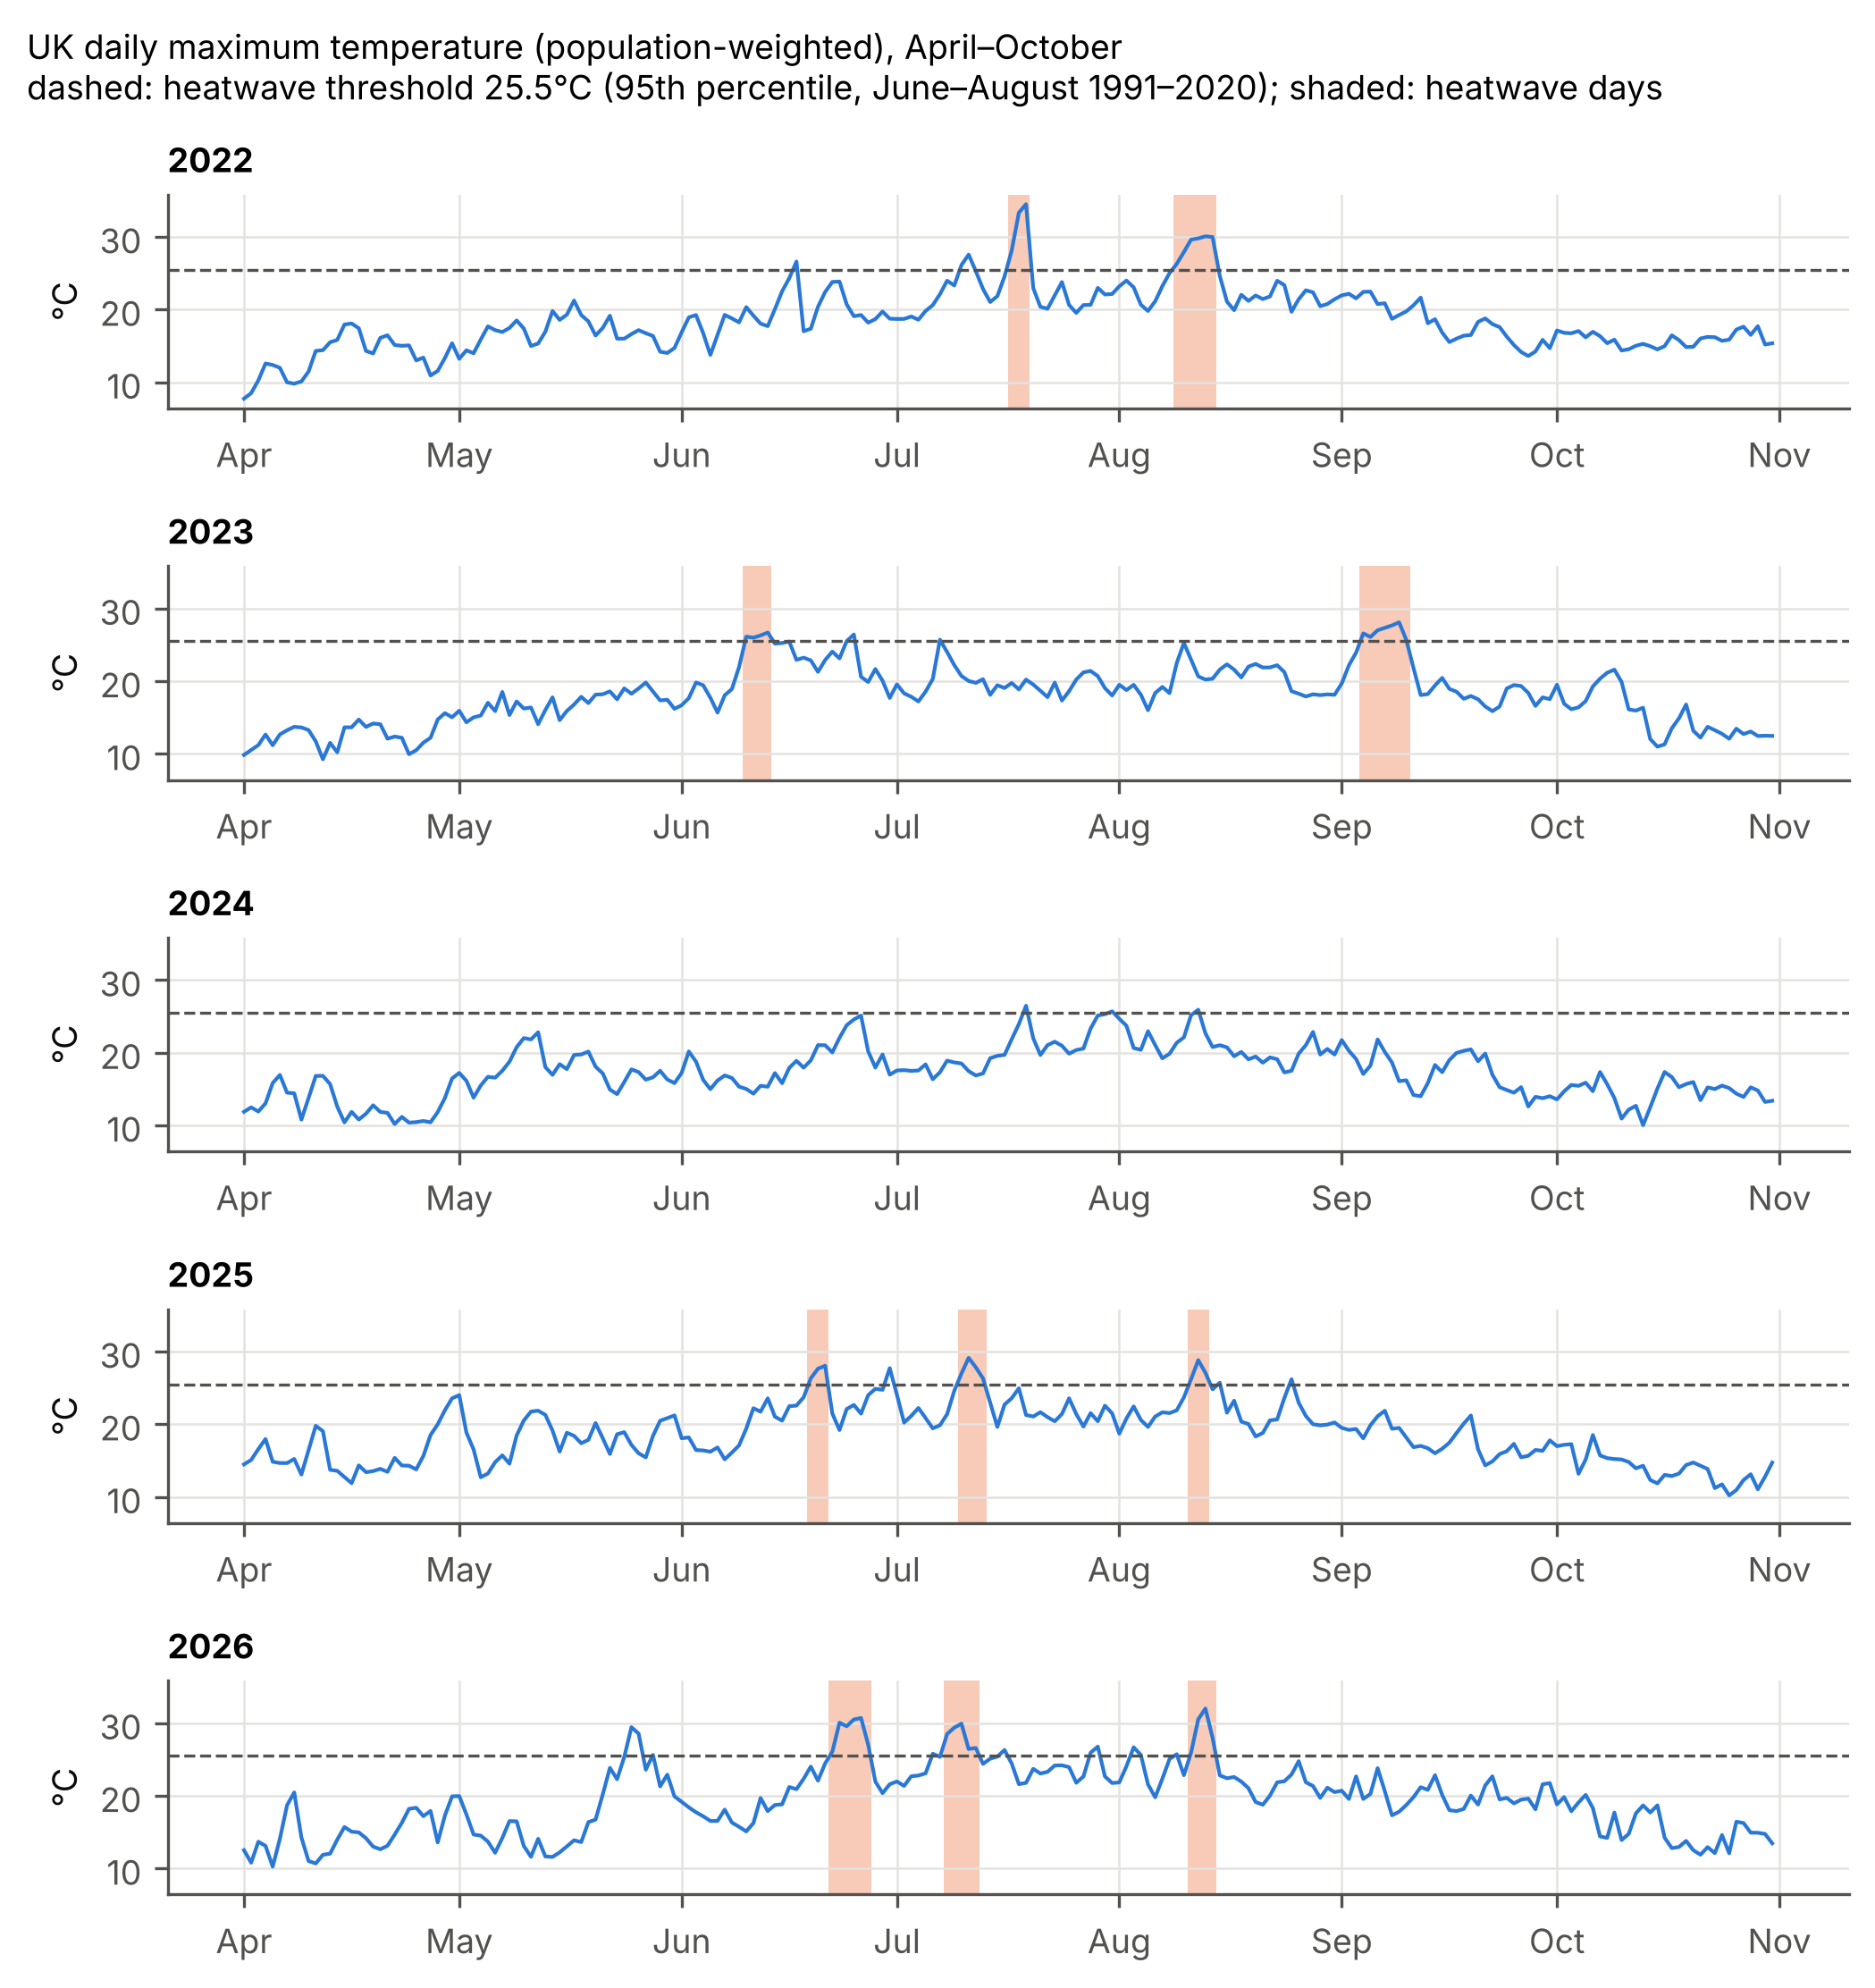
\includegraphics[width=0.82\textwidth]{fig1_heat_timeline.png}
\caption{UK daily maximum temperature, April--October 2022--2026. Shaded days are heatwave days under the pre-registered rule.}
\label{fig:heat}
\end{figure}

\subsection{Attention}

\paragraph{Google Trends.} Weekly search interest for the UK and each nation, 7 November 2021 to 31 October 2026, and daily UK series for each summer. Google Trends reports each request on its own 0--100 scale, so every request includes an anchor term (``dentist'') and each term is expressed as its log ratio to the anchor. Google estimates interest from a sample of searches, so each request was downloaded \NPulls{} times on different days and averaged; between-pull correlations are at least \PullCorrMin{} for every UK series. Terms are grouped into pre-specified families: salience (``heatwave''), coping (``air conditioning'', ``portable air conditioner'', ``heat stroke''), concern (``climate change'', ``global warming'', ``net zero''), and placebo outcomes (``car insurance'', ``recipes'').

\paragraph{Wikipedia.} Daily pageviews of ten pre-specified English Wikipedia articles, globally and, where Wikimedia publishes them, for UK readers only. UK-only figures are withheld on days with few views, and only \WikiUKPass{} of the ten articles (the placebo) is published on enough days to pass the pre-registered coverage rule. The UK-only Wikipedia analysis therefore carries little information, and global pageviews serve as a secondary check.

\section{Design}

\paragraph{Pre-registration.} The analysis plan, including terms, models, hypotheses and decision rules, was committed as the first version of a public repository and archived independently before any outcome data were downloaded. Four deviations were made later. Each is logged with its date and with what had been seen at the time, and each was committed before the analysis it affects was run, except the fourth, which is post hoc and reported as such (Section~\ref{sec:deviations}).

\paragraph{National event study.} For each weekly UK outcome $y_w$,
\begin{equation}
y_w = \sum_{k=-4}^{12} \beta_k\, D_{w-k} + \mu_{\text{week of year}(w)} + \tau_{\text{year}(w)} + \varepsilon_w ,
\end{equation}
where $D_{w-k}$ counts heatwave onsets $k$ weeks before week $w$, the endpoints are binned, and $k=-1$ is the reference. Week-of-year effects compare each heatwave week with the same weeks in other years, and year effects absorb trends. The \emph{impact} is the mean of $\beta_0$ and $\beta_1$. A second model aligns events on the end of each heatwave to measure \emph{decay} (weeks 4--8) and \emph{residue} (weeks 9--12).

\paragraph{Four-nation dose-response.} Using the four nations, attention is regressed on 13 weekly lags of heat dose with nation-by-year, nation-by-week-of-year and week fixed effects. Week effects absorb everything common to the UK in a given week, including national news, so the effect is identified only from differences in heat between nations in the same week.

\paragraph{Inference.} The plan specified Newey--West (national) and Driscoll--Kraay (four-nation) standard errors, together with randomisation inference. A size check on simulated noise, with the same weeks, fixed effects and heatwave timing, shows that the model-based tests reject \SizeAOneMin--\SizeAOneMax\% (national) and \SizeATwo\% (four-nation) of the time at a nominal 5\% level. With so few events these standard errors are not valid, consistent with known problems of inference with few treated units \citep{conley2011,young2019}. The results therefore rest on randomisation inference: the national estimates are compared with \NDraws{} sets of placebo onsets drawn from summer weeks without heat, and the four-nation estimates with all 24 permutations of the nations' heat series. Seven pre-registered hypotheses are tested as one family with Holm's correction \citep{holm1979}, and the ``no residue'' hypotheses use equivalence tests with bounds of $\pm 0.10$ log points \citep{lakens2017}.

\section{Results}

\subsection{A one-week spike}

Figure~\ref{fig:event} shows the weekly estimates. In the week a heatwave begins, searches for ``heatwave'' rise by \ImpSal{} log points (about \ImpSalPct\%; randomisation $p\ImpSalRIEq$). Coping searches rise by \ImpCop{} (about \ImpCopPct\%; $p\ImpCopRIEq$) and concern searches by \ImpCon{} (about \ImpConPct\%; $p\ImpConRIEq$). Global Wikipedia views move the same way: \ImpWikiSal{} for heat articles ($p\ImpWikiSalRIEq$) and \ImpWikiCon{} for climate articles ($p\ImpWikiConRIEq$), although views of the climate articles are already elevated before onset (pre-trend test $p\LeadsWikiConEq$), so that series is weak support. The placebo searches do not move (car insurance \ImpCarIns, $p\ImpCarInsRIEq$; recipes \ImpRecipes, $p\ImpRecipesRIEq$).

The spike is short. By the second week after onset the estimates are back within the range produced by placebo dates. Because the decay is faster than one week, the weekly data cannot identify a half-life, as the plan anticipated; an earlier daily analysis found half-lives of a few days.

\begin{figure}[t]
\centering
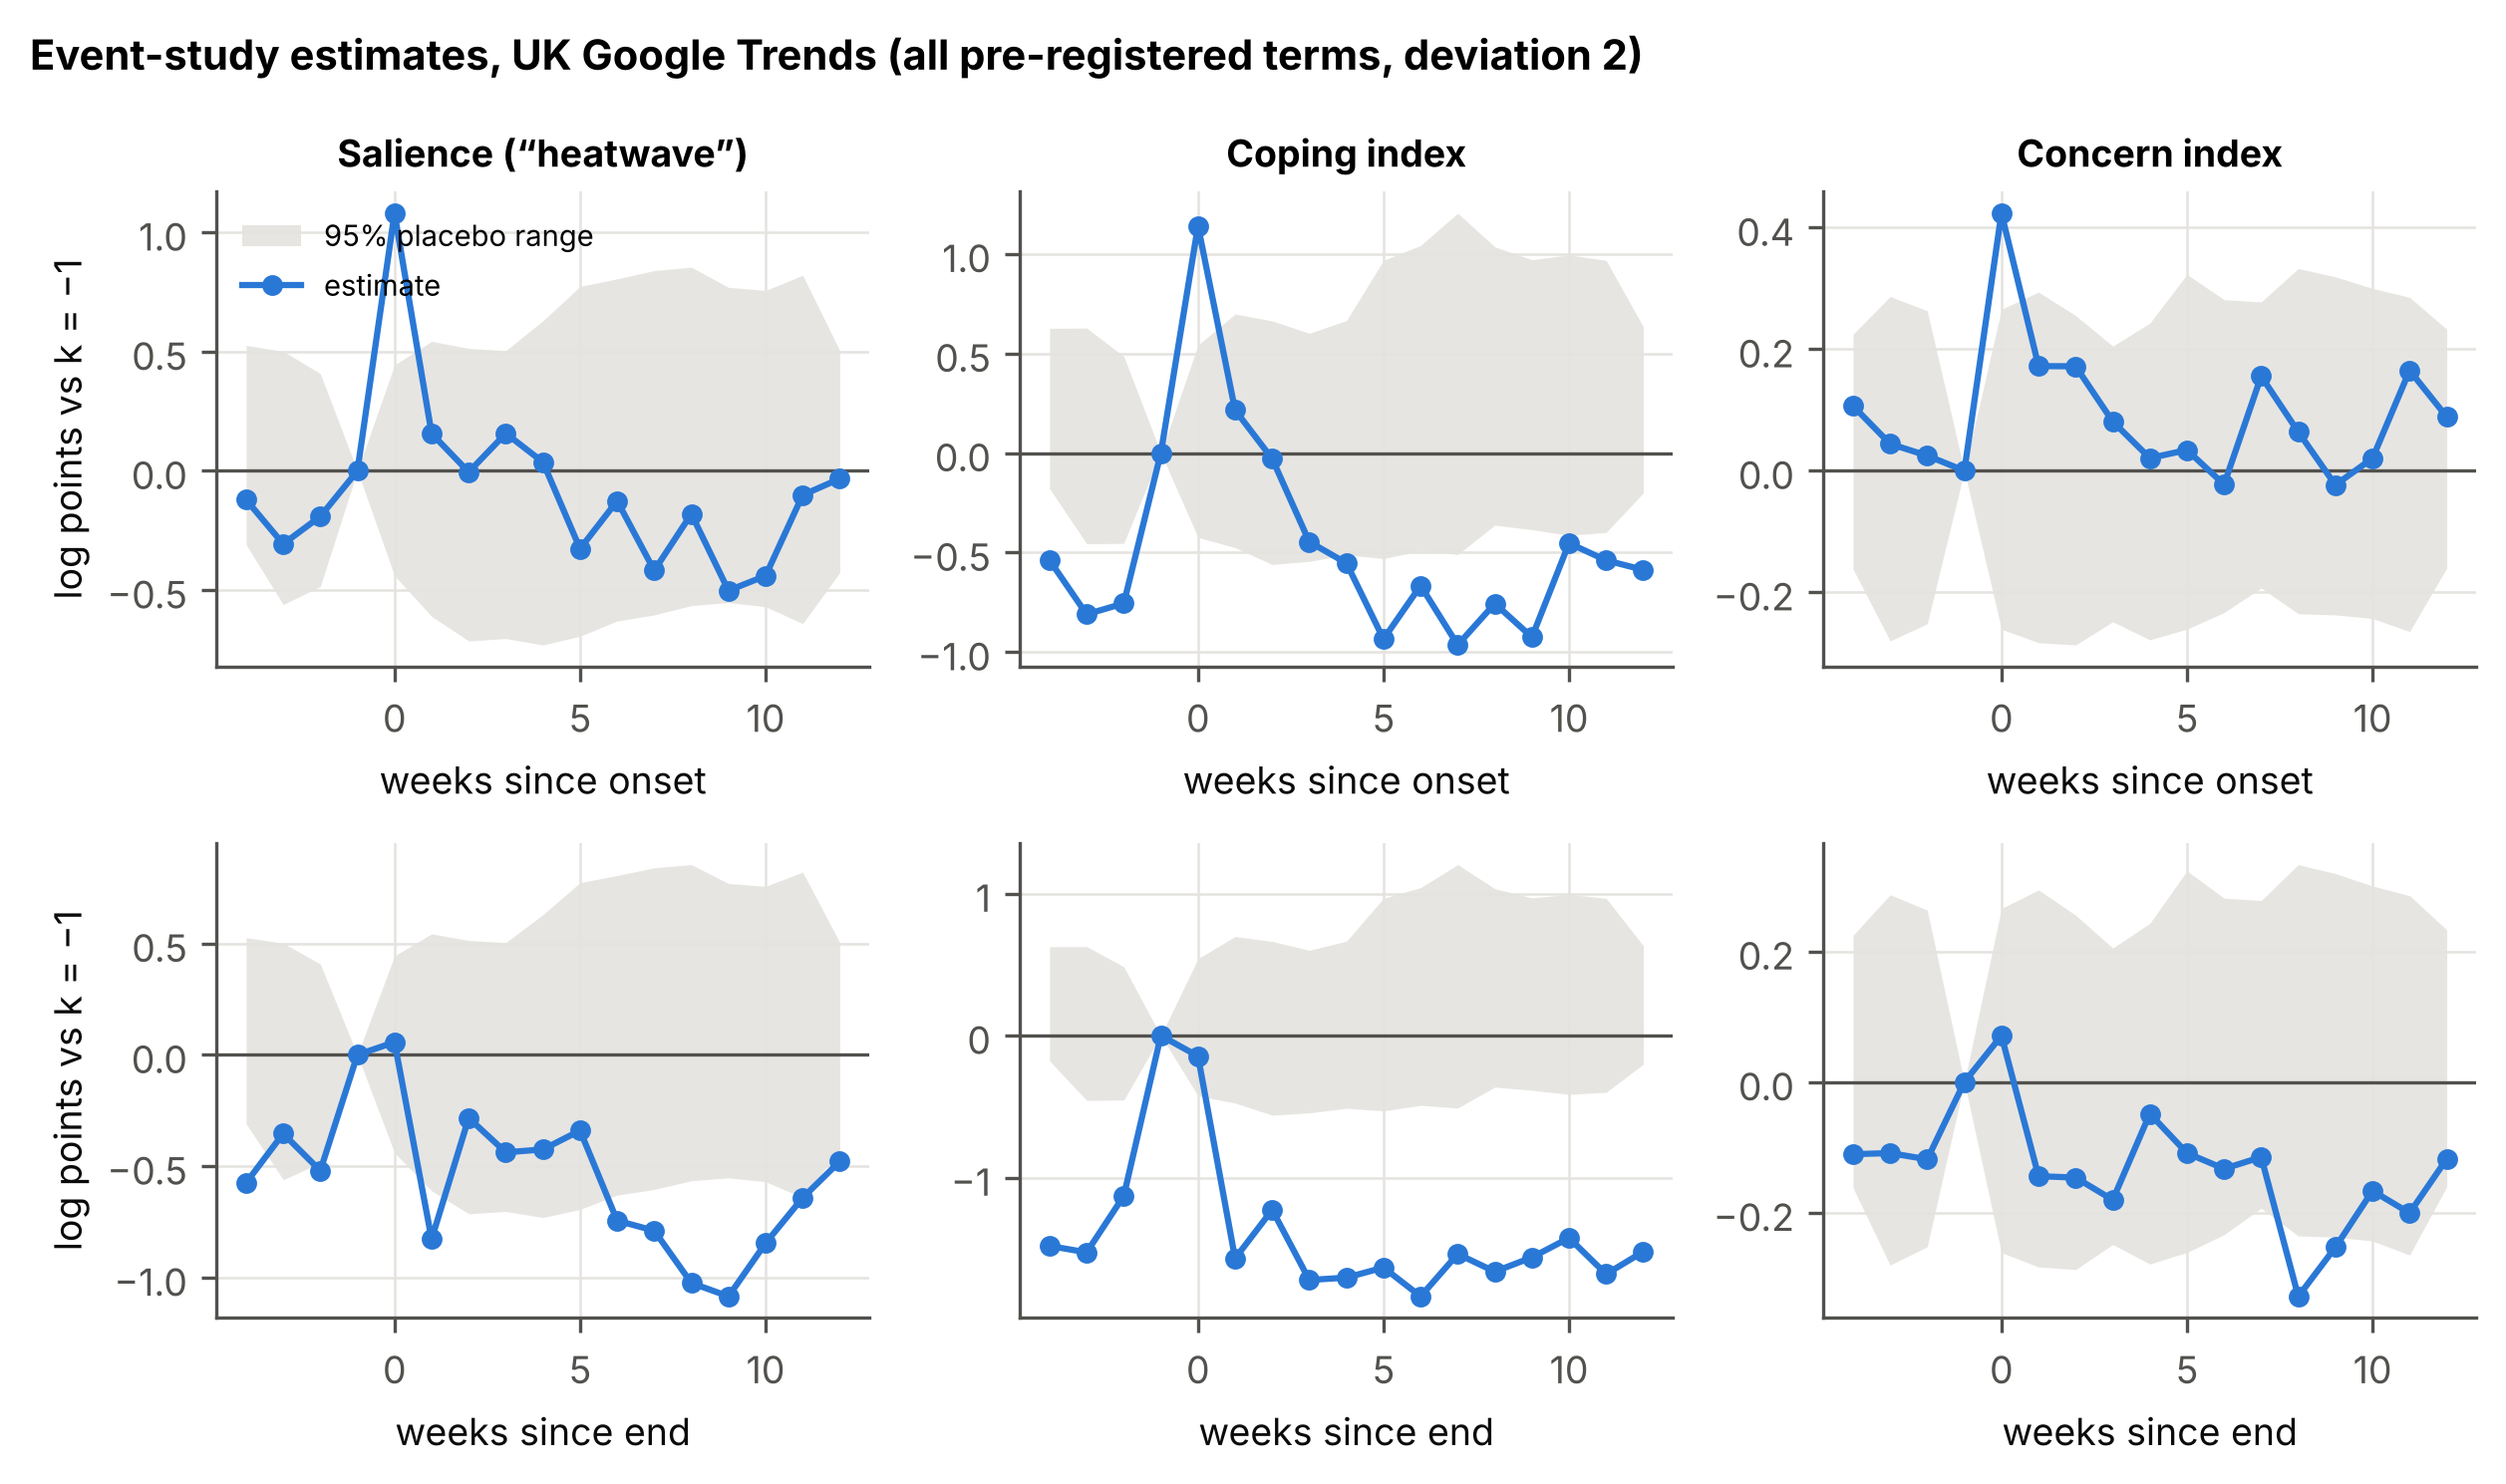
\includegraphics[width=\textwidth]{fig2_event_study_dev2.png}
\caption{Weekly UK search attention around heatwave onsets (top) and ends (bottom), relative to the week before ($k=-1$), with 95\% ranges from \NDraws{} placebo-date draws (grey). All pre-registered terms are used (deviation 2). In the bottom row the reference week often falls inside the heatwave; see Section~\ref{sec:deviations}.}
\label{fig:event}
\end{figure}

\subsection{No lasting residue}

Measured against normal levels (the exploratory estimand of deviation 4), attention two to three months after a heatwave ends is close to zero for every family: \ResSal{} for salience, \ResCop{} for coping and \ResCon{} for concern, with randomisation $p$-values of \ResSalRI, \ResCopRI{} and \ResConRI. The calibrated standard errors (\ResSalSECal, \ResCopSECal, \ResConSECal) are too wide to show formal equivalence within $\pm0.10$ log points, so the data rule out large lasting effects but cannot prove there are none.

\subsection{Pre-registered hypotheses}

Table~\ref{tab:hyp} reports the seven confirmatory tests. With the sparsity rule applied as written, only \NTestablePlan{} of the seven can be tested, and neither shows an effect. With all pre-registered terms (deviation 2) and calibrated inference, \NPresentCal{} of the seven pass after Holm's correction. Under the pre-registered decision rule, which uses the oversized model-based tests in the Holm step, \NPresentPrereg{} would be counted as present (\PresentPreregIDs); I do not interpret these, for the reasons given in the size check. The onset spikes in Figure~\ref{fig:event} are individually clear, but with seven hypotheses and nine events the corrected thresholds are demanding. The four-nation analysis is limited by design: with four nations the smallest attainable randomisation $p$-value is $1/24 \approx 0.042$. Hotter nations show larger coping responses (\DRCop{} log points per 10 degree-days, $p\DRCopRIEq$), but no four-nation estimate can survive the correction. There is no sign that responses weakened after 2022 (coping interaction \HabCop, $p\HabCopRIEq$).

The pre-registered decay and residue estimates (H2, H3) are reported in the table as specified but do not measure what was intended, because their reference week often falls inside the heatwave (Section~\ref{sec:deviations}). The large negative H2 estimate reflects this: it compares attention after the heat with attention during it.

\begin{table}[t]
\centering
\small
\caption{Pre-registered hypotheses. ``Plan'': sparsity rule as written. ``Dev.~2'': all pre-registered terms. $p$ RI: randomisation inference. Calibrated: deviation 3. H1: heat raises salience; H2: coping decays within two months; H3: no concern residue; H4: coping responds more than concern; H5a/b: hotter nations respond more (coping/concern); H6: habituation after 2022.}
\label{tab:hyp}
\resizebox{\textwidth}{!}{\begin{tabular}{llrrrrll}
\toprule
Outcomes & Hyp. & Estimate & $p$ model & $p$ RI & $p$ cal., Holm & Pre-registered rule & Calibrated \\
\midrule
Plan & H1 & -- & -- & -- & -- & not testable & not testable \\
Plan & H2 & -- & -- & -- & -- & not testable & not testable \\
Plan & H3 & $-$0.14 & 0.675 & 0.301 & 0.917 & inconclusive & inconclusive \\
Plan & H4 & -- & -- & -- & -- & not testable & not testable \\
Plan & H5a & -- & -- & -- & -- & not testable & not testable \\
Plan & H5b & 0.13 & 0.093 & 0.458 & 0.917 & not detected & not detected \\
Plan & H6 & -- & -- & -- & -- & not testable & not testable \\
\midrule
Dev.~2 & H1 & 0.62 & 0.009 & 0.012 & 0.087 & present (+) & not detected \\
Dev.~2 & H2 & $-$1.67 & 1.000 & $<$0.001 & 1.000 & undershoot & undershoot \\
Dev.~2 & H3 & $-$0.18 & 0.818 & 0.123 & 1.000 & inconclusive & inconclusive \\
Dev.~2 & H4 & 0.38 & 0.079 & 0.135 & 0.677 & not detected & not detected \\
Dev.~2 & H5a & 0.85 & $<$0.001 & 0.042 & 0.250 & present (+) & not detected \\
Dev.~2 & H5b & 0.32 & $<$0.001 & 0.208 & 0.833 & not detected & not detected \\
Dev.~2 & H6 & $-$0.04 & 0.876 & 1.000 & 1.000 & not detected & not detected \\
\bottomrule
\end{tabular}
}
\end{table}

\subsection{Robustness and placebo checks}

Table~\ref{tab:rob} shows the onset impacts under the pre-registered checks. The salience spike survives dropping weeks with COP summits, the 2024 election and the Queen's death, changing the threshold, and using Met Office dates. The decisive check is the placebo year: moving every heatwave onset to the same week one or two years earlier or later, where there was no heatwave. For ``heatwave'' searches the placebo-year estimates (\PYSalMin{} to \PYSalMax) are all smaller in size than the real effect of \ImpSal. For coping (\PYCopMin{} to \PYCopMax) and concern (\PYConMin{} to \PYConMax), some placebo years produce effects as large as the real ones. Coping searches are strongly seasonal, and the timing of the summer season differs between years in ways that week-of-year effects do not absorb. Under the plan's own criterion, the coping and concern onset effects cannot be reported as causal. The salience effect is the most credible result. In addition, the week before onset is already elevated for coping searches (pre-trend test $p\LeadsCopEq$), consistent with people preparing for forecast heat.

\begin{table}[t]
\centering
\small
\caption{Onset impact (log points) under pre-registered robustness and placebo checks. Placebo-year rows move each heatwave onset to the same week in another year.}
\label{tab:rob}
\begin{tabular}{lrrrr}
\toprule
Check & Salience & Coping & Concern & Placebo (car insurance) \\
\midrule
Main specification & 0.62 & 0.68 & 0.30 & 0.02 \\
Drop COP, election, state-funeral weeks & 0.58 & 0.73 & 0.29 & 0.02 \\
Threshold: 90th percentile & 1.13 & 1.16 & 0.26 & 0.00 \\
Threshold: 97.5th percentile & 0.58 & 0.72 & 0.33 & 0.02 \\
Met Office--documented dates & 0.46 & 0.24 & 0.13 & 0.04 \\
\midrule
Placebo: dates shifted $-2$ years & 0.03 & $-$0.80 & $-$0.26 & $-$0.05 \\
Placebo: shifted $-1$ year & 0.21 & $-$0.72 & $-$0.07 & 0.05 \\
Placebo: shifted $+1$ year & $-$0.04 & 0.46 & 0.30 & $-$0.04 \\
Placebo: shifted $+2$ years & $-$0.37 & 1.04 & $-$0.12 & 0.13 \\
\bottomrule
\end{tabular}

\end{table}

\section{Deviations from the plan}
\label{sec:deviations}

\begin{enumerate}
\item \textbf{Pull dates.} The second and third Google Trends pulls ran two days later than planned. The rule of three pulls on different days, at least 20 hours apart, still holds.
\item \textbf{Sparsity rule.} As written, the rule drops any series with more than 20\% of weeks at a value of 1 or less. Seasonal heat terms sit near zero outside summer (\SparseHeatwave{} of weeks for ``heatwave'', \SparseCopingMin--\SparseCopingMax{} for coping terms), so the rule removed the series the main hypotheses are about. All pre-registered terms are kept in a second, labelled analysis, with a safeguard against floor effects. This was logged before any analysis was run.
\item \textbf{Calibrated inference.} Added after the size check on simulated noise, before any real estimate was produced.
\item \textbf{Reference week (post hoc).} In the end-aligned model the week before the end of a heatwave is often still inside it, so the pre-registered decay and residue compare attention after the heat with attention during it. Baseline-relative estimands were added after provisional results had been seen, and are reported as exploratory.
\end{enumerate}

\section{Discussion}

UK heatwaves produce a sharp but short rise in attention, to the heat itself, to coping with it, and to climate change, and the evidence is most robust for attention to the heat itself. Attention returns to normal within one to two weeks, and there is no detectable residue months later. In issue-attention terms, each heatwave is a brief spike rather than a step change, and there is no sign that the record summer of 2022 or the longer 2026 heatwave changed this pattern.

Three limitations matter. First, nine events give little statistical power, and the main confirmatory tests do not pass after correction. Second, search data measure attention, not beliefs or behaviour: a week of searches about heat and climate change may or may not change what people think or do. Third, the placebo-year failures show that seasonal patterns in coping and concern searches are not fully absorbed by the design, so those effects should be read as descriptive.

The obvious next step is to turn the study around: to state predictions before the summer of 2027 and test them as heatwaves happen, rather than looking back. Daily data would also allow the decay to be measured properly.

\paragraph{Data and code.} All data, code, the pre-registration and the deviation log are at \url{https://github.com/TheAlchemist108/heat-leaves-a-mark}. Contains modified Copernicus Climate Change Service information (2026). HadUK-Grid data are \copyright{} Crown copyright, Met Office, under the Open Government Licence.

\begin{thebibliography}{99}
\setlength{\itemsep}{2pt}\small
\bibitem[Conley and Taber(2011)]{conley2011} Conley, T.~G. and Taber, C.~R. (2011). Inference with ``difference in differences'' with a small number of policy changes. \emph{Review of Economics and Statistics}, 93(1), 113--125.
\bibitem[Debnath et al.(2023)]{debnath2023} Debnath, R., Bardhan, R. and Bell, M.~L. (2023). Lethal heatwaves are challenging India's sustainable development. \emph{PLOS Climate}, 2(4), e0000156.
\bibitem[Downs(1972)]{downs1972} Downs, A. (1972). Up and down with ecology: the ``issue-attention cycle''. \emph{The Public Interest}, 28, 38--50.
\bibitem[Egan and Mullin(2012)]{egan2012} Egan, P.~J. and Mullin, M. (2012). Turning personal experience into political attitudes: the effect of local weather on Americans' perceptions about global warming. \emph{Journal of Politics}, 74(3), 796--809.
\bibitem[Hersbach et al.(2020)]{hersbach2020} Hersbach, H. et al. (2020). The ERA5 global reanalysis. \emph{Quarterly Journal of the Royal Meteorological Society}, 146, 1999--2049.
\bibitem[Hollis et al.(2019)]{hollis2019} Hollis, D., McCarthy, M., Kendon, M., Legg, T. and Simpson, I. (2019). HadUK-Grid: a new UK dataset of gridded climate observations. \emph{Geoscience Data Journal}, 6(2), 151--159.
\bibitem[Holm(1979)]{holm1979} Holm, S. (1979). A simple sequentially rejective multiple test procedure. \emph{Scandinavian Journal of Statistics}, 6(2), 65--70.
\bibitem[Konisky et al.(2016)]{konisky2016} Konisky, D.~M., Hughes, L. and Kaylor, C.~H. (2016). Extreme weather events and climate change concern. \emph{Climatic Change}, 134, 533--547.
\bibitem[Lakens(2017)]{lakens2017} Lakens, D. (2017). Equivalence tests: a practical primer for t tests, correlations, and meta-analyses. \emph{Social Psychological and Personality Science}, 8(4), 355--362.
\bibitem[Lang(2014)]{lang2014} Lang, C. (2014). Do weather fluctuations cause people to seek information about climate change? \emph{Climatic Change}, 125, 291--303.
\bibitem[Moore et al.(2019)]{moore2019} Moore, F.~C., Obradovich, N., Lehner, F. and Baylis, P. (2019). Rapidly declining remarkability of temperature anomalies may obscure public perception of climate change. \emph{Proceedings of the National Academy of Sciences}, 116(11), 4905--4910.
\bibitem[Sisco et al.(2017)]{sisco2017} Sisco, M.~R., Bosetti, V. and Weber, E.~U. (2017). When do extreme weather events generate attention to climate change? \emph{Climatic Change}, 143, 227--241.
\bibitem[Young(2019)]{young2019} Young, A. (2019). Channeling Fisher: randomization tests and the statistical insignificance of seemingly significant experimental results. \emph{Quarterly Journal of Economics}, 134(2), 557--598.
\end{thebibliography}

\end{document}
